\documentclass{article}
\usepackage[a4paper, total={6in, 9in}]{geometry} 
\usepackage{amsmath} 
\usepackage{graphicx}
\usepackage{float}
\usepackage{listingFreeFem}

\lstset{
	columns=fullflexible,
	frame=shadowbox,
	numbers=left,
	numberstyle=\color{gray},
	breaklines=true,
	postbreak=\mbox{\textcolor{red}{$\hookrightarrow$}\space},
}
\newcommand{\Vol}{\rotatebox[origin=c]{180}{\ensuremath{A}}}

\title{Incompressible Inviscid Flow using FreeFEM++} 
\author{Gaurav Gupta} 
\date{\today} 

% The preamble ends with the command \begin{document}
\begin{document} % All begin commands must be paired with an end command somewhere
\maketitle % creates title using information in preamble (title, author, date)
\section{Governing Equations}
Incompressible inviscid flow is simulated by solving the govering equations in FreeFEM++
using artifical compressibility method. For 2D flow, the mesh is created in FreeFEM++, whereas
in 3D flow, the mesh is created with GMSH and imported in FreeFEM++.
\subsection*{Continuity Equation}
$$\nabla \cdot \vec{u}  = 0$$

\subsection*{Momentum Equation}
$$ \frac{\partial{\vec{u}}}{\partial{t}} + (\vec{u} \cdot \nabla) \vec{u} = - \nabla P $$

\noindent Note: The density ($\rho$) is taken as one for simplicity.

\subsection*{Boundary Conditions}
\begin{table}[H]
    \centering
    \begin{tabular}{||c|c||}
        \hline
        \textbf{Boundary} & \textbf{Type}                  \\
        \hline
        Inlet             & Dirchlet ($\vec{u}$ = [1 0 0]) \\
        \hline
        Domain Walls      & Free-slip                      \\
        \hline
        Cylinder Wall     & Free-slip                      \\
        \hline
    \end{tabular}
\end{table}
\section{Artificial Compressibility Method}
The artificial compressibility method is used to solve incompressible flow
equations with as hyperbolic equations in a time-marching fashion like compressible
flow equations. It is achieved by introducing an artificial parameter in the continuity
equation in terms of presssure related through a constant $\beta$.

\subsection*{Modified Continuity Equation}
$$\beta \frac{\partial{p}}{\partial{t}} + \nabla \cdot \vec{u}  = 0$$

\subsection*{Momentum Equation}
$$ \frac{\partial{\vec{u}}}{\partial{t}} + (\vec{u} \cdot \nabla) \vec{u} = - \nabla P $$

\noindent The set of equations are solved until a steady solution is obtained. This steady solution
is also the solution of the original govering equations as $\frac{\partial{p}}{\partial{t}}$ tends
to 0 at steady state.\\

\subsection*{Weak Form}
The time derivatives are written using Forward Euler and the weak form is derived
for the above modified equations.

$$\int_{\Omega} \left( \frac{\vec{u}^{n+1}\cdot\vec{v}}{\Delta t} + (\vec{u}^{n+1} \cdot \nabla\vec{u}^{n+1})\cdot\vec{v} - p\nabla \cdot\vec{v} - q\nabla \cdot \vec{u}^{n+1}
    - \frac{\beta p^{n+1} q}{\Delta t}\right) d\Vol - \int_{\Omega} \left(\frac{\vec{u}^{n}\cdot\vec{v}}{\Delta t} - \frac{\beta p^{n} q}{\Delta t}\right) d\Vol = 0$$

\noindent The non-linear term of the equation is computed using the inbuilt \emph{convect} function of FreeFEM++.

\begin{lstlisting}[language=FreeFem, caption=Problem definition in FreeFEM++]

    solve GE([u1,u2,p],[v1,v2,q])
   =int2d(Th)
   ([u1,u2]'*[v1,v2]/dt
   -div(v)*p
   -div(u)*q
   -Beta*p*q/dt
   )
   +int2d(Th)(
   -(con(un,dt)'*[v1,v2])/dt
   +Beta*pn*q/dt   
   )
   +on(1, u1=1, u2=0)
   +int1d(Th,qft=qf1pTlump,5)(1e10*(u1*normalappx+u2*normalappy)*(v1*normalappx+v2*normalappy))
   +on(3, u2=0)
   +on(4, u2=0);
\end{lstlisting}

\section{Results of 2D Computation}
The code is tested using the benchmark case of flow around a cylinder. The solution of the flow is already known
from potential flow theory. $\beta$ is a user-defined parameter whose value is varied along with the number of points
on the cylinder boundary. An initial domain of [-10D,10D] in x and [-6D, 6D] in y-direction. The unstructured
mesh used for computation is presented in \textbf{Figure \ref{fig:mesh}}.

\subsection{Number of points on cylinder}
The number of points on the cylinder surface is increased from 50 to 150 in three steps. The variation in
pressure distribution over the surface and residual is computed and plotted in \textbf{Figure \ref{fig:n}}.
The residual magnitude decreases with increase in the number of points but the trend remains unchanged. On
increasing the number of points from 50 to 100, we see significant improvement in the pressure at top and
bottom point on the surface whereas the increase from 100 to 150 has very little effect on pressure distribution.
On the contrary, with increase in number of points little improvement is observed on the pressure at stagnation
point.
\begin{figure}[H]
    \centering
    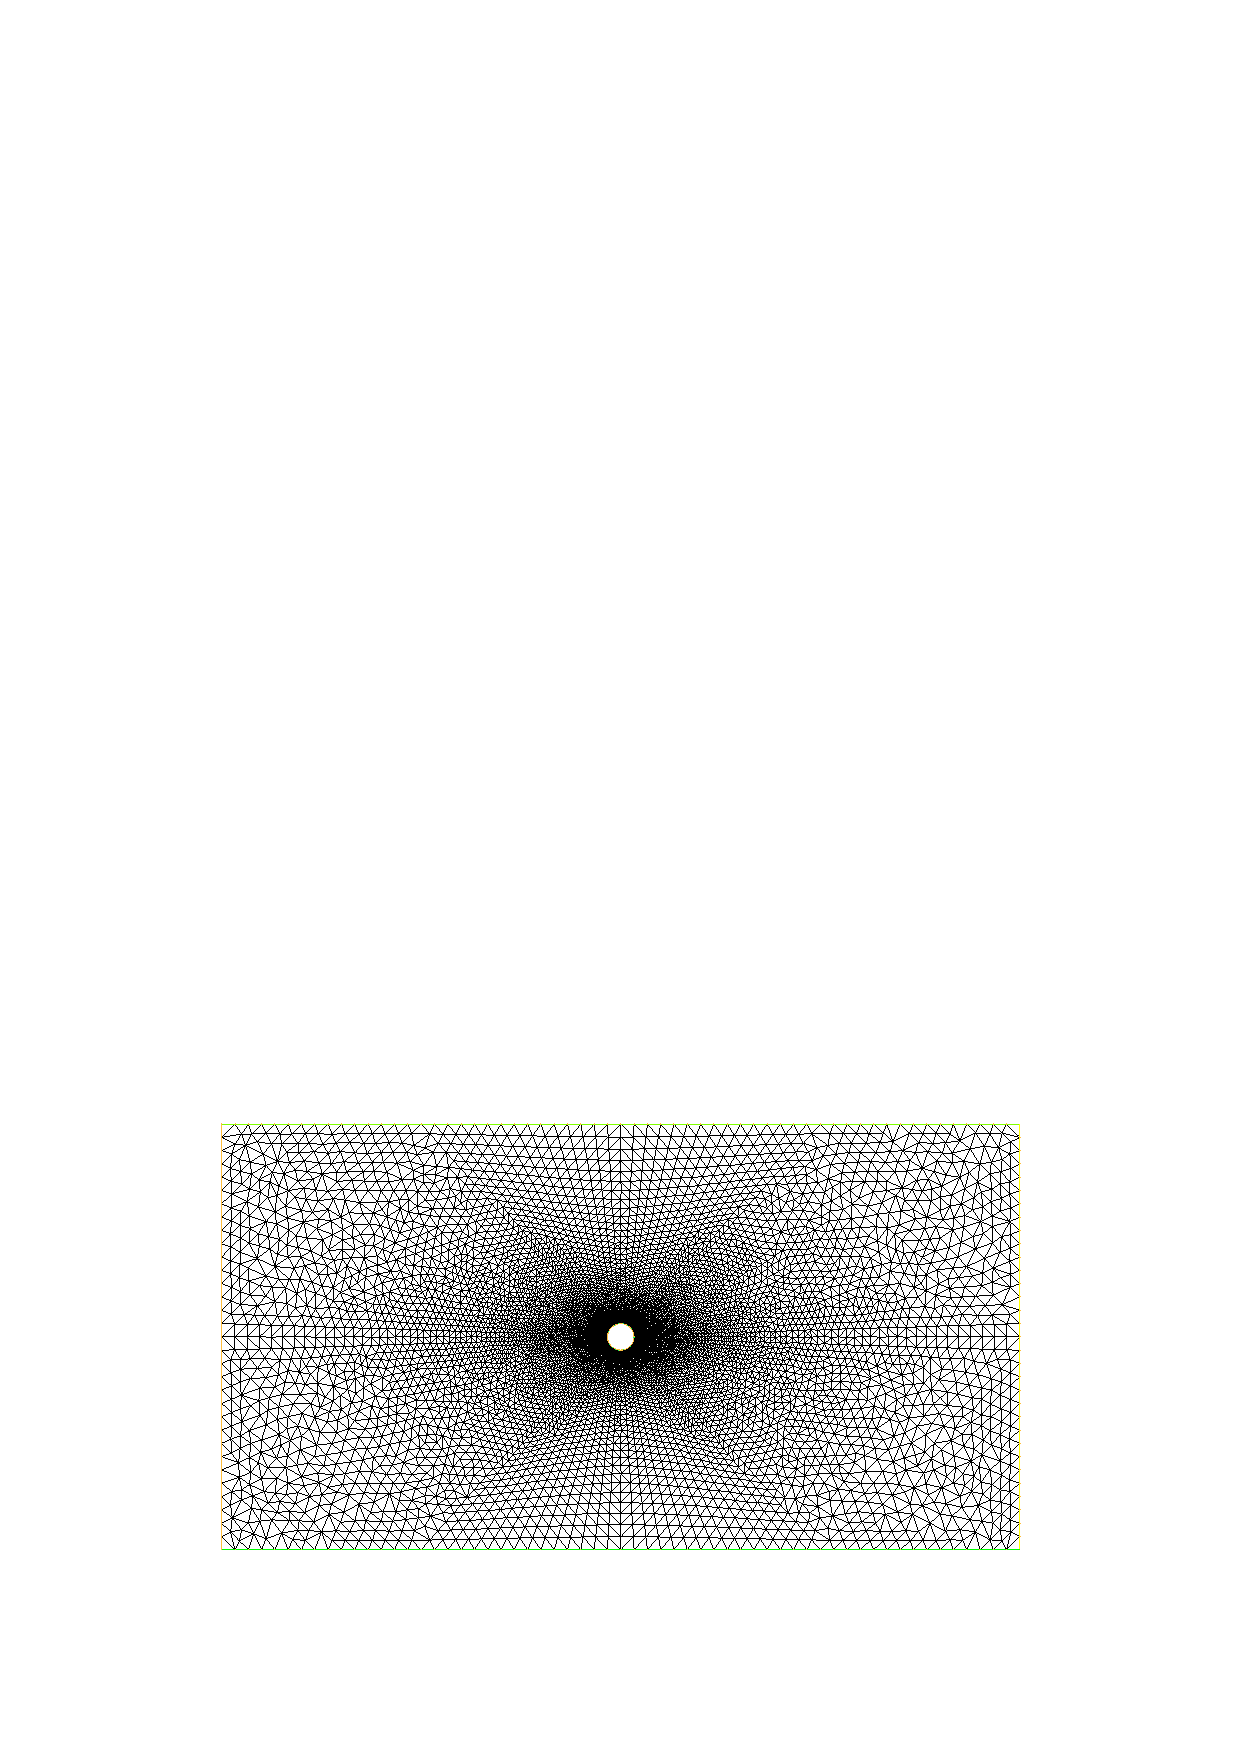
\includegraphics[width=\textwidth]{mesh.png}
    \caption{Unstructured mesh contructed in FreeFEM++ with 100 points on the cylinder body}
    \label{fig:mesh}
\end{figure}
\begin{figure}[H]
    \centering
    \includegraphics[width=\textwidth]{../n.png}
    \caption{Variation in the residual and pressure distribution over the surface with time for different number of points on the cylinder boundary}
    \label{fig:n}
\end{figure}

\begin{figure}[H]
    \centering
    \includegraphics[width=0.95\textwidth]{../cyl_n.png}
    \caption{Velocity contour over the cylinder for the three cases.}
    \label{fig:cyl_n}
\end{figure}

\subsection{Variation of $\beta$}
$\beta$ is the user-defined parameter to control the artifical compressibility introduced in the equation. In general, the value of $\beta$ is choosen
less than one and a smaller value helps in faster convergence. In our case, we test with three values of $\beta$ and we observe that reducing the value
from $10^{-5}$ to $10^{-7}$ had no effect on the residual but decreasing it further to $10^{-9}$ caused an increase in the magnitude of residual.
The decrease in value of $\beta$ has negligible effect on the pressure distribution as all the three curves approximately coincide with each other
(\textbf{Figure \ref{fig:b}}).

\begin{figure}[H]
    \centering
    \includegraphics[width=0.95\textwidth]{../b.png}
    \caption{Variation in the residual and pressure distribution over the surface with time for different value of $\beta$.}
    \label{fig:b}
\end{figure}

\begin{figure}[H]
    \centering
    \includegraphics[width=0.95\textwidth]{../cyl_b.png}
    \caption{Velocity contour over the cylinder for the three cases.}
    \label{fig:cyl_b}
\end{figure}

\subsection{Variation with Domain}
The dependence of solution with domain size is tested by reducing the domain to [-5D,5D] in x and [-4D, 4D] in y from the initial size
and then increasing it to [-15D, 15D] in x and [-10D, 10D] in y. The cell size on domain boundaries and cylinder surface is kept constant
for all the domains. For the largest domain of $30\times16$, a sharp decrease in residual is observed with the least residual compared to
other domain sizes. The pressure distribution is approximately similar in all the domains as the plots coincide with each other
(\textbf{Figure \ref{fig:d}}).

\begin{figure}[H]
    \centering
    \includegraphics[width=0.95\textwidth]{../d.png}
    \caption{Variation in the residual and pressure distribution over the surface with time for domain.}
    \label{fig:d}
\end{figure}

\begin{figure}[H]
    \centering
    \includegraphics[width=0.95\textwidth]{../cyl_d.png}
    \caption{Velocity contour over the cylinder for the three cases.}
    \label{fig:cyl_d}
\end{figure}

\end{document} % This is the end of the document